\documentclass[11pt]{article}
\usepackage[a4paper,margin=1in]{geometry}
\usepackage[T1]{fontenc}
\usepackage{mathptmx}
\usepackage{microtype}
\usepackage{amsmath}
\usepackage{booktabs}
\usepackage{graphicx}
\usepackage{xcolor}
\usepackage{enumitem}
\usepackage[hidelinks]{hyperref}
\usepackage{caption}
\captionsetup{font=small,labelfont=bf}
\setlist{nosep,leftmargin=*}

\newcommand{\pass}{\textbf{PASS}}
\newcommand{\fail}{\textbf{FAIL}}
\newcommand{\inc}{\textbf{INCONCLUSIVE}}
\newcommand{\mirage}{\textbf{MIRAGE}}

\title{\textbf{Emergent Intelligence, Defined So It Can Fail:}\\[2pt]
A Pre-registered Test in AI Agents\\ That Invent Their Own Language}
\author{Amit Brahmbhatt\\[2pt]
\small Quantum Clarity LLC, Milpitas, California, USA\\
\small ORCID: \href{https://orcid.org/0009-0003-5882-8476}{0009-0003-5882-8476}}
\date{\small Preprint, version 1.0 \textbullet{} 31 October 2026\\
DOI: \href{https://doi.org/10.5281/zenodo.23849135}{10.5281/zenodo.23849135}}

\begin{document}
\maketitle

\begin{abstract}
\noindent
``Emergent'' is used loosely for capabilities that nobody designed. We propose an operational
definition that can fail. A capability is emergent with respect to its designer specification to
the degree that it meets five criteria: it goes beyond the training objective (C1), keeps
developing after convergence (C2), is caused by interaction at equal compute (C3), comes with
self-organized structure above an untrained baseline (C4), and, if it appears to switch on with
scale, survives continuous metrics (C5). A system receives an \emph{EI profile} of
\pass/\fail/\inc{} verdicts rather than a label. We implement the criteria in EI-Bench, an
open harness, and apply it to populations of neural agents that invent a discrete language in a
reconstruction game. Every threshold was pre-registered in a public git history before the runs
that test it. Across four rounds and 256 runs on one GPU, the profile is: C1 \pass{}
(held-out accuracy 0.90--0.99 on unseen attribute combinations); C2 \pass{}, replicated three
times; C3 \fail{}, including with heterogeneous populations; C4 \fail{} at 20 seeds; and the
apparent capability jump with model size is a metric \mirage{} (per-attribute transition
2.6$\times$ wider than the exact-match transition). A shrink-and-perturb control shows that
the turnover effect is not explained by restored plasticity. Forcing newcomers to relearn the
language from the population improves it (+0.19 held-out accuracy, 95\% CI [0.004, 0.409]),
whereas restoring fresh-scale weights while keeping latent knowledge does not. In this system,
emergence came from generations, not crowds. We report two places where our pre-registered
wording overclaimed or needed tightening, and how we handled them.
\end{abstract}

\begin{center}
\fbox{\begin{minipage}{0.92\linewidth}\small
\textbf{Plain-language summary.}
People call today's AI ``artificial'', but many of its abilities were never programmed by anyone;
they appeared on their own. We asked whether that kind of ``emergence'' can be tested honestly,
in a way that could also come out negative. We wrote down five checks and built small AI agents
that must invent their own code words to describe objects to each other. Before every experiment
we published our pass/fail rules, like sealing a prediction in an envelope before the result is
known. The agents invented working languages that correctly describe objects they had never seen.
An apparent sudden leap in ability as the agents got bigger turned out to be an illusion of how
we scored them. Putting more agents in conversation did not make them better. But regularly
replacing agents with newcomers, who had to learn the language from the others, steadily improved
it, much as human languages are refined as each generation learns them. Giving old agents a
``refresh'' without that relearning did not help. In short: in this system, emergence came from
generations, not crowds. The same checks can now be applied to AI systems in use today, such as
teams of AI assistants working together.
\end{minipage}}
\end{center}

\section{Introduction}

``Artificial intelligence'' names where intelligence comes from: it is built. It says nothing
about \emph{how} capabilities arise. In modern learning systems many abilities are not written
down by anyone; they follow from scale, data and interaction. ``Emergent intelligence'' would be
a better description, but only if it means something specific. A word that every system
qualifies for is useless, and claims of emergence are known to be fragile: abrupt ``emergent
abilities'' of language models \cite{wei2022} can be artefacts of discontinuous metrics
\cite{schaeffer2023}.

We therefore treat emergence as an empirical property with a falsifiable test. Our contributions:
\begin{enumerate}
  \item \textbf{An operational definition} with five criteria and explicit verdict rules,
        reported as a profile rather than a label (Section~\ref{sec:def}).
  \item \textbf{EI-Bench}, an open, single-GPU harness that implements the criteria for
        populations of communicating agents, with batched population training, turnover and
        perturbation controls, and bootstrap statistics (Section~\ref{sec:methods}).
  \item \textbf{A pre-registered, four-round study} of 256 runs, with thresholds committed to git
        before each round (Section~\ref{sec:results}). The profile it yields is C1 \pass,
        C2 \pass, C3 \fail, C4 \fail, C5 \mirage.
  \item \textbf{A mechanism result for C2}: generational turnover improves emergent languages
        through cultural transmission, not through restored plasticity.
\end{enumerate}

\section{Related work}

\textbf{Emergent communication.} Agents trained to coordinate through a discrete channel develop
conventions in the sense of Lewis signalling games \cite{lewis1969}. Chaabouni et al.\
\cite{chaabouni2020} showed that such languages can generalize to unseen attribute combinations
without being compositional, and introduced the positional and bag-of-symbols disentanglement
measures we use. Rita et al.\ \cite{rita2022} found that population effects depend on
heterogeneity among agents.

\textbf{Iterated learning.} When a language must be relearned by each new generation, transmission
favours structure that is easy to learn \cite{kirby2008}. Our turnover manipulation is a neural
version of this idea.

\textbf{Emergent abilities and metrics.} Wei et al.\ \cite{wei2022} documented abilities that
appear abruptly with scale; Schaeffer et al.\ \cite{schaeffer2023} argued many are produced by
non-linear or discontinuous metrics. Our C5 criterion operationalizes that critique.

\textbf{Plasticity.} Deep networks lose the ability to learn under continued training
\cite{dohare2024}; re-initialization and shrink-and-perturb \cite{ash2020} restore it. Any
benefit of agent turnover must be separated from this effect, which is what our C2c control does.

\section{An operational definition}\label{sec:def}

Let a system $S$ be produced by a designer specification $D = $ (architecture, objective, data,
training procedure). A capability of $S$ is \emph{emergent with respect to $D$} to the degree
that it meets the criteria in Table~\ref{tab:criteria}.

\begin{table}[h]
\centering\small
\begin{tabular}{@{}lp{0.68\linewidth}@{}}
\toprule
Criterion & Question \\
\midrule
C1 Beyond the objective & Does $S$ do something $D$ never rewarded? \\
C2 Ongoing emergence & Does $S$ keep developing after convergence, beyond more of the same training? \\
C3 Interaction as source & Is part of the capability caused by interaction among agents, at equal compute? \\
C4 Self-organized structure & Does unspecified structure form, above an untrained baseline? \\
C5 Jumps survive smooth metrics & If a capability seems to switch on with scale, does the jump hold under continuous metrics? \\
\bottomrule
\end{tabular}
\caption{The five criteria. Each receives a verdict; together they form the system's EI profile.}
\label{tab:criteria}
\end{table}

\textbf{Verdicts.} Seeds are the unit of replication. We report means with 95\% percentile
bootstrap confidence intervals over seeds (10{,}000 resamples). A test is \pass{} when the whole
interval clears its threshold, \inc{} when only the mean does, and \fail{} otherwise; C5 adds
\mirage{} and NO-JUMP outcomes. A two-sided Mann--Whitney $U$ test is reported as a secondary
statistic that is robust to outlier seeds.

\textbf{Pre-registration.} Every round's design, thresholds and verdict rules were written into
\texttt{DEFINITION.md} and committed to a public git repository before any run of that round.
Earlier verdicts are never re-scored; follow-up questions receive new, separately named tests
(C2 $\rightarrow$ C2b $\rightarrow$ C2c).

\section{Testbed and methods}\label{sec:methods}

\textbf{Task.} Objects have $A{=}4$ attributes with $V{=}8$ values each (4{,}096 objects). A
sender maps an object to a message of $L{=}6$ symbols from a vocabulary of $K{=}16$; a receiver
must reconstruct every attribute from the message alone. Ten percent of attribute combinations
(410 objects) are held out from training, while every individual value still appears in training.
Nothing in $D$ specifies the language, its structure, or what any symbol means.

\textbf{Agents.} Senders and receivers are GRU networks (hidden size 128, embedding 32 unless
swept). Symbols are discrete in the forward pass and trained with straight-through
Gumbel-softmax ($\tau{=}1$). Populations use stacked parameters with a leading agent dimension,
so a population of $N$ senders and $N$ receivers trains as one set of batched matrix
multiplications.

\textbf{Training.} Adam (learning rate $10^{-3}$), batch 256, 8{,}000 steps, with linear
learning-rate decay to $0.05\times$ over the last 20\% of steps. In \emph{mixed} populations,
sender--receiver pairings are re-drawn every step; in the \emph{isolated} control, each sender
keeps one receiver. Both use identical parameters and compute.

\textbf{Turnover (C2).} Mixed populations with $N{=}4$ train for 24{,}000 steps. From step
8{,}000 until 85\% of training, every 500 steps one randomly chosen agent (sender or receiver)
is replaced by a freshly initialized agent and its Adam state is cleared (24 events per run).
The learning rate decays over the final 15\%. The C2 metric is the change in held-out accuracy
from step 8{,}000 (the start of the turnover phase) to the end, compared against an arm without turnover.

\textbf{Controls.} \emph{C2b} (v0.2) adds isotropic Gaussian noise whose norm matches the
displacement a reset would cause. \emph{C2c} (v0.3) applies shrink-and-perturb
\cite{ash2020}: $w' = \lambda w + \sigma f$, with $f$ a fresh initialization sample,
$\sigma{=}0.1$ and $\lambda = \|f\|/\|w\|$ per parameter tensor, so the agent returns to
fresh-init scale while keeping the direction of its learned weights.

\textbf{Metrics.} C1: exact-match accuracy on held-out combinations (chance $2.4\times10^{-4}$).
C3: held-out accuracy, scored over all $N^2$ pairings for mixed populations and own pairs only
for isolated ones, a comparison that deliberately favours the control. C4: topographic
similarity (Spearman correlation of pairwise meaning and message Hamming distances, 1{,}000
objects), and positional and bag-of-symbols disentanglement \cite{chaabouni2020}, each compared
with the same agents before training; a \pass{} needs topsim gain $>0.05$ and posdis or bosdis
gain $>0.05$. C5: model size is swept and exact-match accuracy is compared with per-attribute
accuracy (Section~\ref{sec:c5}).

\textbf{Compute.} All runs used one NVIDIA RTX 5090 under WSL2 with PyTorch 2.15 (CUDA 13.2),
with up to six worker processes sharing a lock-file work queue. Summed training time was
136~min (v0, 46 runs), 934~min (v0.2, 160 runs) and 531~min (v0.3, 50 runs).

\section{Results}\label{sec:results}

Table~\ref{tab:profile} summarizes all scored tests. Seeds were 0--4 (v0), 100--109 (v0.2) and
200--219 (v0.3), never reused.

\begin{table}[t]
\centering\small
\begin{tabular}{@{}llll@{}}
\toprule
Round & Test & Verdict & Key number (mean [95\% CI]) \\
\midrule
v0 (5 seeds) & C1 & \pass & held-out acc.\ 0.993 [0.981, 1.000] \\
 & C2 & \pass & $\Delta_\text{turnover}-\Delta_\text{none}$ = 0.108 [0.032, 0.210] \\
 & C3 & \fail & mixed $-$ isolated = $-$0.020 [$-$0.053, 0.010] \\
 & C4 & \inc & posdis gain 0.070 [0.033, 0.105] \\
 & C5 & \inc & jump ratios 0.58 (exact), 0.31 (per-attribute) \\
\midrule
v0.2 (10 seeds) & C1 & \pass & 0.970 [0.941, 0.993] \\
 & C2 & \pass & 0.076 [0.033, 0.133]; MW $p$ = 0.001 \\
 & C2b & \pass$^\dagger$ & $\Delta_\text{reset}-\Delta_\text{perturb}$ = 0.896 [0.813, 0.963] \\
 & C3b & \fail & heterogeneous: $-$0.012 [$-$0.221, 0.135] \\
 & C4 & \inc & posdis gain 0.076 [0.040, 0.112] \\
 & C5b & \mirage & width ratio $R$ = 2.63 [1.99, 3.80] \\
\midrule
v0.3 & C1 (20 seeds) & \pass & 0.899 [0.800, 0.975] \\
 & C2 (10 seeds) & \pass & 0.233 [0.069, 0.443]; MW $p$ = 0.017 \\
 & C2c (10 seeds) & \pass & $\Delta_\text{reset}-\Delta_\text{S\&P}$ = 0.190 [0.004, 0.409]; MW $p$ = 0.045 \\
 & C4 (20 seeds) & \fail & posdis gain 0.039 [0.021, 0.058] \\
\bottomrule
\end{tabular}
\caption{All scored verdicts. $^\dagger$See Section~\ref{sec:deviations} on what C2b can and
cannot show.}
\label{tab:profile}
\end{table}

\subsection{C1: generalization beyond the objective}
Single sender--receiver pairs reconstruct held-out combinations almost as well as trained ones
(held-out/train ratio 0.95--0.99), at roughly 4{,}000 times chance. In v0.3, 2 of 20 pairs did not
converge (0.195, 0.444), which lowers the mean but not the verdict. This is the weak form of C1:
generalization to unseen combinations of familiar parts.

\subsection{C4: structure is real but not disentangled}
Topographic similarity rises reliably above the untrained baseline in every round (gain
0.114--0.152). Positional disentanglement improves too, but stays below the pre-registered
0.05 margin: \inc{} at 5 and 10 seeds and \fail{} at 20 seeds (gain 0.039 [0.021, 0.058]);
bag-of-symbols disentanglement shows no gain. As in \cite{chaabouni2020}, the languages generalize
well without being cleanly compositional.

\subsection{C5: the capability jump is a metric mirage}\label{sec:c5}
v0.2 swept 12 hidden sizes from 4 to 256 (5 seeds each). Exact-match accuracy appears to switch on
between sizes 32 and 96 (Figure~\ref{fig:c5}). Per-attribute accuracy, a continuous measure of the
same predictions, rises steadily over the whole range. The 10--90\% transition widths are 1.44
octaves for exact match and 3.78 octaves for per-attribute accuracy, a ratio of 2.63 [1.99, 3.80],
which meets the pre-registered \mirage{} rule ($R \geq 2$ with the CI lower bound above 1.5).
Because exact match requires all four attributes to be correct, it compresses a gradual
improvement into an apparent jump, as argued in \cite{schaeffer2023}.

\begin{figure}[t]
\centering
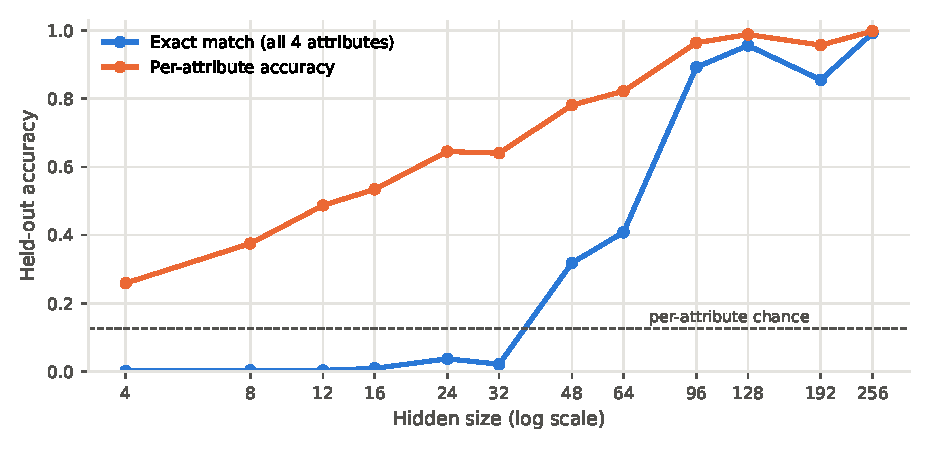
\includegraphics[width=0.92\linewidth]{fig_c5b.pdf}
\caption{C5b. Held-out accuracy versus hidden size (mean of 5 seeds per size). The apparent jump
in exact match (blue) corresponds to a gradual rise in per-attribute accuracy (orange).}
\label{fig:c5}
\end{figure}

\subsection{C3: interaction within a generation adds nothing}
Mixed populations reliably converge on a shared language: senders and receivers that never trained
as a fixed pair understand each other (cross-play accuracy 0.82--0.96, against 0 for isolated
pairs). This does not count towards C3, because the mixed objective requires it. On the capability
that C3 scores, held-out generalization, mixed populations are no better than isolated pairs at
equal compute: not with homogeneous agents (v0: $-$0.020; v0.2 replicate: $-$0.016), and not when
agents learn at different speeds (v0.2 C3b, learning-rate multipliers from 0.5 to 2:
$-$0.012 [$-$0.221, 0.135]). At $N{=}8$, mixing even made languages less disentangled
(posdis $-$0.052 [$-$0.076, $-$0.026], secondary).

\subsection{C2: turnover improves languages, through transmission}
Replacing agents during training improved held-out accuracy relative to continued training in all
three rounds (Table~\ref{tab:profile}). The no-turnover arm tends to drift after convergence, and
some seeds collapse (to 0.426 in v0.2 and 0.118 in v0.3), while turnover arms mostly end near 1.0.

\textbf{Is it disruption?} v0.2 compared turnover with a perturbation of matched size. Perturbed
populations collapsed (final accuracy 0.066), which made C2b pass by a wide margin. A post-hoc diagnostic on a separately trained population
showed why: matched noise left the perturbed agent's weights about 1.5$\times$ larger than its
trained weights, with an output layer about 9$\times$ larger than at initialization, so its symbol
choices saturated and it largely stopped learning. C2b thus showed that re-initialization beats an
equal-sized disruption, but not \emph{why}.

\textbf{Is it restored plasticity?} v0.3 compared turnover with shrink-and-perturb, which returns
the agent to fresh-init scale while keeping its learned direction (in the experiment runs, averaged
over 240 events: weight norm 0.44 of the pre-intervention agent's, cosine 0.945 to its old weights). A calibration run before any v0.3
experiment confirmed the intended contrast: shrink-and-perturb brought weight norm to 0.50 of the
trained agent's (0.49 for a reset); the agent's accuracy with its partners fell to 0.02 but recovered
to 0.53 within 50 steps, against 0.07 for a reset. Its knowledge
was latent, not lost.

The result (Figure~\ref{fig:c2c}): turnover beat shrink-and-perturb by 0.190 [0.004, 0.409]
(\pass, Mann--Whitney $p = 0.045$), and shrink-and-perturb did no better than no turnover at all
(final accuracy 0.771 vs.\ 0.728, $p = 0.79$). Turnover also produced more structured languages than
shrink-and-perturb (topsim gain difference 0.046 [0.004, 0.093]). Under the pre-registered reading,
relearning the language from the population adds something that restored plasticity does not. This
is what iterated learning predicts \cite{kirby2008}. The effect is real at this sample size but its
lower confidence bound is close to zero, and it is partly driven by control seeds that collapse.

\begin{figure}[t]
\centering
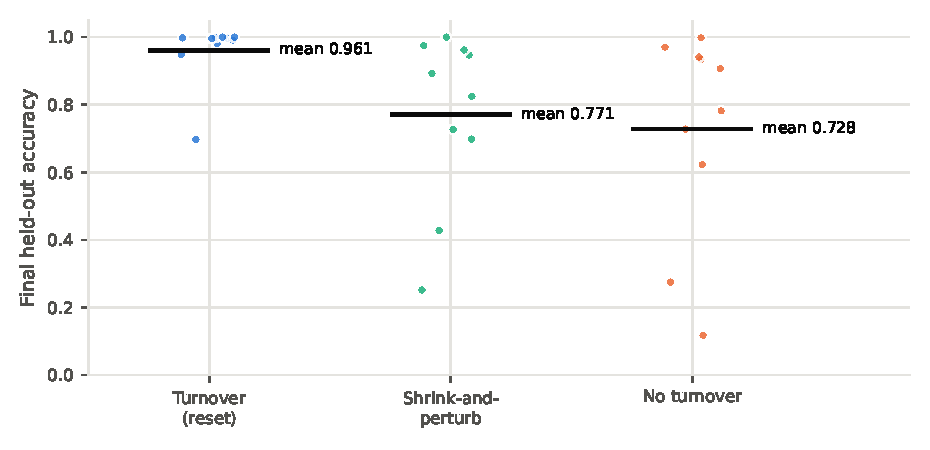
\includegraphics[width=0.92\linewidth]{fig_c2c.pdf}
\caption{C2c. Final held-out accuracy per seed (10 seeds per arm, $N{=}4$, 24{,}000 steps).
Turnover ends near 1.0; shrink-and-perturb and no turnover are statistically indistinguishable.}
\label{fig:c2c}
\end{figure}

\section{Deviations, corrections and incidents}\label{sec:deviations}

We list every departure from the pre-registered plan, because the method's value depends on it.
\begin{enumerate}
  \item \textbf{C2b wording overclaimed.} The v0.2 pre-registration said a C2b \pass{} would mean
        ``the gain comes from relearning the language from others''. The post-hoc saturation check
        showed C2b cannot support that reading. The verdict stands; the wording is retained in the
        record and explicitly corrected in the results (\texttt{DEFINITION.md} \S8). The question
        was carried into v0.3.
  \item \textbf{C2c design was calibrated, and its reading tightened, before any run.} A first
        calibration showed that shrink-and-perturb destroys immediate function, which raised the
        question of whether it was a valid control. A recovery test showed knowledge is retained in
        latent form; this calibration was written into the pre-registration. The rule for reading
        an equivalence result was extended from ``FAIL with the CI inside $[-0.03, 0.03]$'' to any
        non-\pass{} with that CI, before any v0.3 run. A proposed ``reset all agents'' arm was
        dropped before running, with the reason recorded.
  \item \textbf{One worker crash.} In v0.2 one of six worker processes died from a transient CUDA
        driver error. Results are written only when a run completes, and a stale lock is reclaimed,
        so the interrupted run was redone in full by another worker; all 160 runs completed. Workers
        restart themselves automatically from v0.3 on.
\end{enumerate}

\section{Limitations}

This is a deliberately small system. ``Beyond the objective'' here is compositional
generalization, a weak form of C1. Results come from one task, one architecture family and one
channel size, and C3 was tested only for pairings re-drawn every step. Thresholds such as the
0.05 disentanglement margin are conventions we fixed in advance, not natural constants. With 10
seeds, C2c has limited precision; a larger replication would sharpen the effect size. Finally, a
profile describes a system, not intelligence in general: the criteria are intended to be applied
to other systems, where the verdicts may differ.

\section{Conclusion and future work}

An operational, pre-registered definition of emergence is practical on a single GPU, and it
discriminates: in this system it returned two passes, two failures and one mirage. The clearest
positive finding is about mechanism. Capability improved when the language had to be passed to new
learners, and did not improve when agents merely interacted more or regained plasticity. The next
step applies the same harness and criteria to societies of language-model agents with persistent
memory, running under a deterministic runtime authority layer that records tamper-evident
evidence, to ask whether the same profile appears in systems that are deployed today.

\section*{Data and code availability}
Code (Apache-2.0), the full pre-registration history and all reports are in EI-Bench,
\url{https://github.com/amitb-quantum/ei-bench}. All 256 per-run result files, the scored reports and the
pre-registration history are included as a dataset file in this Zenodo record.

\section*{Acknowledgements}
Experiment design, code and drafting were carried out with the assistance of an AI system
(Claude, Anthropic). All experiments were run, checked and approved by the author, who takes
responsibility for the content.

\begin{thebibliography}{9}\small
\bibitem{ash2020} J.~T. Ash and R.~P. Adams. On warm-starting neural network training.
  \emph{NeurIPS}, 2020.
\bibitem{chaabouni2020} R.~Chaabouni, E.~Kharitonov, D.~Bouchacourt, E.~Dupoux and M.~Baroni.
  Compositionality and generalization in emergent languages. \emph{ACL}, 2020.
\bibitem{dohare2024} S.~Dohare, J.~F. Hernandez-Garcia, Q.~Lan, P.~Rahman, A.~R. Mahmood and
  R.~S. Sutton. Loss of plasticity in deep continual learning. \emph{Nature}, 632:768--774, 2024.
\bibitem{kirby2008} S.~Kirby, H.~Cornish and K.~Smith. Cumulative cultural evolution in the
  laboratory: an experimental approach to the origins of structure in human language.
  \emph{PNAS}, 105(31):10681--10686, 2008.
\bibitem{lewis1969} D.~Lewis. \emph{Convention: A Philosophical Study}. Harvard University
  Press, 1969.
\bibitem{rita2022} M.~Rita, F.~Strub, J.-B. Grill, O.~Pietquin and E.~Dupoux. On the role of
  population heterogeneity in emergent communication. \emph{ICLR}, 2022.
\bibitem{schaeffer2023} R.~Schaeffer, B.~Miranda and S.~Koyejo. Are emergent abilities of large
  language models a mirage? \emph{NeurIPS}, 2023.
\bibitem{wei2022} J.~Wei et al. Emergent abilities of large language models.
  \emph{Transactions on Machine Learning Research}, 2022.
\end{thebibliography}

\end{document}
